\section{Experiments}
\label{sec:experiments}

This section presents the empirical evaluation of \textsc{SenseMath}.
We describe the experimental setup (\S\ref{sec:exp_setup}), report the main prompting asymmetry (\S\ref{sec:main_result}), per-category analysis (\S\ref{sec:per_category}), strict-prompt validation (\S\ref{sec:strict}), and CoT strategy analysis (\S\ref{sec:cot_strategy}).

% ─────────────────────────────────────────────────────────────────────────────
\subsection{Experimental Setup}
\label{sec:exp_setup}

\paragraph{Models.}
We evaluate five instruction-tuned models spanning three families:
Qwen3-30B and Qwen3-8B \citep{qwen2025qwen3},
Llama-3.1-8B-Instruct \citep{grattafiori2024llama},
and GPT-4o-mini and GPT-4.1-mini \citep{openai2024gpt4o}.
GPT-4.1-mini is a more capable successor to GPT-4o-mini that achieves near-ceiling CoT accuracy on \textsc{SenseMath} at $d{=}4$, providing an important reference point for how strong baseline performance constrains the prompting asymmetry.
Open-weight models are served via vLLM with tensor parallelism; GPT models are accessed through the OpenAI API.
All inferences use greedy decoding (temperature$\,{=}\,0$) and $\texttt{max\_tokens}{=}512$.

\paragraph{Conditions.}
Each of the 1{,}600 item families is evaluated under three prompting conditions (CoT, NS, Strict) across three variants (strong, weak, control), yielding $1{,}600 \times 3 \times 3 = 14{,}400$ inferences per model and \textbf{72{,}000 total inferences} across five models.

\paragraph{Metrics.}
Our primary analysis compares accuracy on strong-shortcut versus control items under NS and CoT prompting, supplemented by the NS rate (shortcut strategy classification by GPT-4.1-mini judge) and the normalised improvement metric defined in \S\ref{sec:metrics}.

% ─────────────────────────────────────────────────────────────────────────────
\subsection{Main Result: Prompting Asymmetry at $d{=}4$}
\label{sec:main_result}

Table~\ref{tab:main_results} presents per-condition accuracies on strong-shortcut and control items across all four digit scales for five models.

\begin{table*}[t]
  \centering
  \small
  \setlength{\tabcolsep}{2.5pt}
  \caption{Per-condition results across digit scales for five models. Acc = accuracy; NS\% = shortcut-strategy rate classified by GPT-4.1-mini judge. $S$ = strong-shortcut variant, $W$ = weak-shortcut variant, $C$ = control variant. All numbers are percentages (rounded to integers).}
  \label{tab:main_results}
  \begin{tabular}{ll|rrr|rrr|rrr|rrr}
    \toprule
    \textbf{Model} & \textbf{Metric} & \multicolumn{3}{c|}{$d=2$ (\%)} & \multicolumn{3}{c|}{$d=4$ (\%)} & \multicolumn{3}{c|}{$d=8$ (\%)} & \multicolumn{3}{c}{$d=16$ (\%)} \\
     &  & $S$ & $W$ & $C$ & $S$ & $W$ & $C$ & $S$ & $W$ & $C$ & $S$ & $W$ & $C$ \\
    \midrule
    GPT-4o-mini & $\text{Acc}_{\text{CoT}}$ & 88 & 88 & 85 & 78 & 70 & 65 & 75 & 62 & 55 & 67 & 53 & 46 \\
     & $\text{Acc}_{\text{NS}}$ & 92 & 92 & 87 & 84 & 72 & 63 & 82 & 73 & 62 & 70 & 59 & 51 \\
     & $\text{NS\%}_{\text{CoT}}$ & 28 & 18 & 24 & 27 & 16 & 18 & 36 & 21 & 22 & 37 & 27 & 22 \\
     & $\text{NS\%}_{\text{NS}}$ & 46 & 37 & 44 & 77 & 65 & 78 & 84 & 76 & 80 & 90 & 80 & 90 \\
    \midrule
    GPT-4.1-mini & $\text{Acc}_{\text{CoT}}$ & 99 & 99 & 99 & 88 & 89 & 76 & 80 & 72 & 65 & 74 & 58 & 60 \\
     & $\text{Acc}_{\text{NS}}$ & 100 & 100 & 100 & 96 & 94 & 83 & 95 & 86 & 83 & 86 & 70 & 69 \\
     & $\text{NS\%}_{\text{CoT}}$ & 16 & 7 & 7 & 20 & 4 & 1 & 46 & 22 & 37 & 57 & 34 & 48 \\
     & $\text{NS\%}_{\text{NS}}$ & 70 & 58 & 62 & 68 & 50 & 70 & 80 & 66 & 78 & 87 & 86 & 87 \\
    \midrule
    Qwen3-8B & $\text{Acc}_{\text{CoT}}$ & 97 & 99 & 98 & 74 & 70 & 65 & 70 & 62 & 59 & 56 & 48 & 50 \\
     & $\text{Acc}_{\text{NS}}$ & 98 & 98 & 95 & 72 & 55 & 53 & 70 & 55 & 52 & 56 & 38 & 34 \\
     & $\text{NS\%}_{\text{CoT}}$ & 30 & 17 & 14 & 37 & 16 & 25 & 55 & 26 & 44 & 56 & 36 & 46 \\
     & $\text{NS\%}_{\text{NS}}$ & 66 & 56 & 55 & 86 & 72 & 88 & 87 & 79 & 90 & 90 & 88 & 98 \\
    \midrule
    Qwen3-30B-A3B & $\text{Acc}_{\text{CoT}}$ & 100 & 100 & 98 & 68 & 58 & 56 & 57 & 44 & 47 & 48 & 30 & 31 \\
     & $\text{Acc}_{\text{NS}}$ & 100 & 100 & 100 & 73 & 68 & 56 & 74 & 50 & 52 & 60 & 42 & 44 \\
     & $\text{NS\%}_{\text{CoT}}$ & 26 & 15 & 15 & 39 & 22 & 33 & 60 & 39 & 47 & 59 & 42 & 52 \\
     & $\text{NS\%}_{\text{NS}}$ & 86 & 77 & 76 & 86 & 84 & 92 & 89 & 84 & 83 & 94 & 96 & 98 \\
    \midrule
    Llama-3.1-8B & $\text{Acc}_{\text{CoT}}$ & 82 & 76 & 80 & 66 & 70 & 58 & 62 & 53 & 51 & 51 & 36 & 33 \\
     & $\text{Acc}_{\text{NS}}$ & 74 & 70 & 68 & 59 & 56 & 55 & 57 & 48 & 50 & 55 & 45 & 42 \\
     & $\text{NS\%}_{\text{CoT}}$ & 26 & 24 & 25 & 31 & 25 & 24 & 37 & 24 & 24 & 40 & 33 & 26 \\
     & $\text{NS\%}_{\text{NS}}$ & 62 & 58 & 59 & 78 & 76 & 69 & 86 & 82 & 90 & 92 & 87 & 86 \\
    \bottomrule
  \end{tabular}
\end{table*}


The key pattern across models is an asymmetric response to NS prompting: on strong-shortcut items, NS either maintains or slightly improves accuracy relative to CoT, whereas on control items NS consistently reduces accuracy.
For GPT-4o-mini at $d{=}4$, NS raises strong-shortcut accuracy to 84.5\% (vs.\ 78.2\% under CoT) while control accuracy drops from 64.8\% to 63.0\%.
Qwen3-8B shows a more nuanced pattern: strong accuracy holds steady (74.2\%$\to$72.0\%) while control drops (65.0\%$\to$53.2\%).
GPT-4.1-mini shows a large NS improvement on strong items (87.8\%$\to$96.5\%) while control also improves but less so (76.5\%$\to$83.2\%), reflecting near-ceiling capacity.
Qwen3-30B shows NS improving both strong and control, but with a larger boost on strong items (68.0\%$\to$72.8\% vs.\ 55.5\%$\to$56.5\%).
Llama-3.1-8B is the exception: NS degrades accuracy on strong items (66.5\%$\to$59.0\%) while control changes minimally (57.8\%$\to$54.8\%).

Bootstrap 95\% confidence intervals (10,000 resamples) for the strong-vs-control accuracy differential confirm that the asymmetry is reliable for GPT-4o-mini (+0.080 [+0.015, +0.147]) and Qwen3-8B (+0.095 [+0.032, +0.158]), while GPT-4.1-mini (+0.020 [$-$0.035, +0.075]), Qwen3-30B (+0.037 [$-$0.020, +0.095]), and Llama-3.1-8B ($-$0.045 [$-$0.125, +0.035]) include zero.

\paragraph{Dose-response pattern.}
The weak-shortcut variant provides an intermediate condition between strong and control.
At $d{=}4$ under NS, all five models show accuracy ordered as \{strong, weak\} $>$ control: GPT-4o-mini (84.5\%, 71.8\%, 63.0\%), GPT-4.1-mini (96.5\%, 94.0\%, 83.2\%), Qwen3-8B (72.0\%, 54.8\%, 53.2\%), Qwen3-30B (72.8\%, 68.5\%, 56.5\%), and Llama-3.1-8B (59.0\%, 56.0\%, 54.8\%).
In all cases, the gap between shortcut-bearing variants (strong and weak) and the control variant is substantially larger than the gap between strong and weak themselves.
This pattern is consistent with the mechanism identified by the strategy-use analysis: NS induces shortcut attempts on all items, and accuracy reflects whether a viable shortcut exists (strong and weak) or not (control).

\begin{figure*}[t]
\centering
\small
\fbox{\parbox{0.96\textwidth}{%
\textbf{Case 1: magnitude\_estimation} (Qwen3-8B, $d{=}4$) \hfill \textit{Answer: (A) 103{,}020{,}000}\\
\textit{Which is the best estimate for $10100 \times 10200$?} \quad (A) 103020000 \quad (B) 103020010 \quad (C) 103020020 \quad (D) 103019990\\[4pt]
%
\textbf{CoT response} (wrong, picks C):\\
{\footnotesize\ttfamily
We are asked to estimate the value of: $10^{100} \times 10^{200}$\\
Step 1: Use the properties of exponents. $10^a \times 10^b = 10^{a + b}$. So: $10^{100} \times 10^{200} = 10^{300}$\\
Step 2: Compare with the answer choices: (A) $10^{3020000}$ (B) $10^{3020010}$ (C) $10^{3020020}$ (D) $10^{3019990}$\\
Wait --- this is not the same as $10^{300}$! These choices are way too large. There's a misinterpretation\ldots\\
\mbox{}\hfill[\textit{continues for 1{,}275 tokens, eventually picks C}]}\\[4pt]
%
\textbf{NS response} (correct, picks A):\\
{\footnotesize\ttfamily
We are asked to estimate: $10100 \times 10200$\\
Step 1: Both numbers are close to 10{,}000. Write as: $10100 = 10000 + 100$, $10200 = 10000 + 200$\\
$(10000 + 100)(10000 + 200) = 10000^2 + 10000 \times 300 + 100 \times 200 = 100{,}000{,}000 + 3{,}000{,}000 + 20{,}000 = 103{,}020{,}000$\\
\mbox{}\hfill$\boxed{A}$}\\[4pt]
\textit{Analysis:} CoT misparses ``10100'' as $10^{100}$ (an exponent), leading to 1{,}275 tokens of confused reasoning. NS reads the integers correctly and applies FOIL decomposition in 3 steps.
}}
\caption{Case study: CoT fails but NS succeeds (Qwen3-8B, magnitude\_estimation, strong-shortcut, $d{=}4$). Actual model output shown verbatim. CoT misparses integers as exponents; NS decomposes correctly.}
\label{fig:case_study}
\end{figure*}

The $d{=}4$ scale appears to occupy a ``sweet spot'' where problems are difficult enough that CoT computation is error-prone, yet the digit scale is small enough that shortcut strategies remain executable.
At $d{=}2$, problems are sufficiently easy that both conditions yield similar accuracy.
At $d{=}8$ and $d{=}16$, the asymmetry persists for GPT-4o-mini and Qwen3-8B but becomes inconsistent for other models, suggesting that larger digit scales introduce model-specific fragilities in shortcut execution.

% ─────────────────────────────────────────────────────────────────────────────
\subsection{Per-Category Analysis (Exploratory)}
\label{sec:per_category}

The aggregate accuracy pattern masks substantial variation across shortcut types. The following per-category analysis is exploratory; we report descriptive patterns without category-level significance tests.
Figure~\ref{fig:bar_d4} shows per-category accuracy on strong-shortcut items under CoT and NS prompting at $d{=}4$ for all five models.

\begin{figure*}[t]
    \centering
    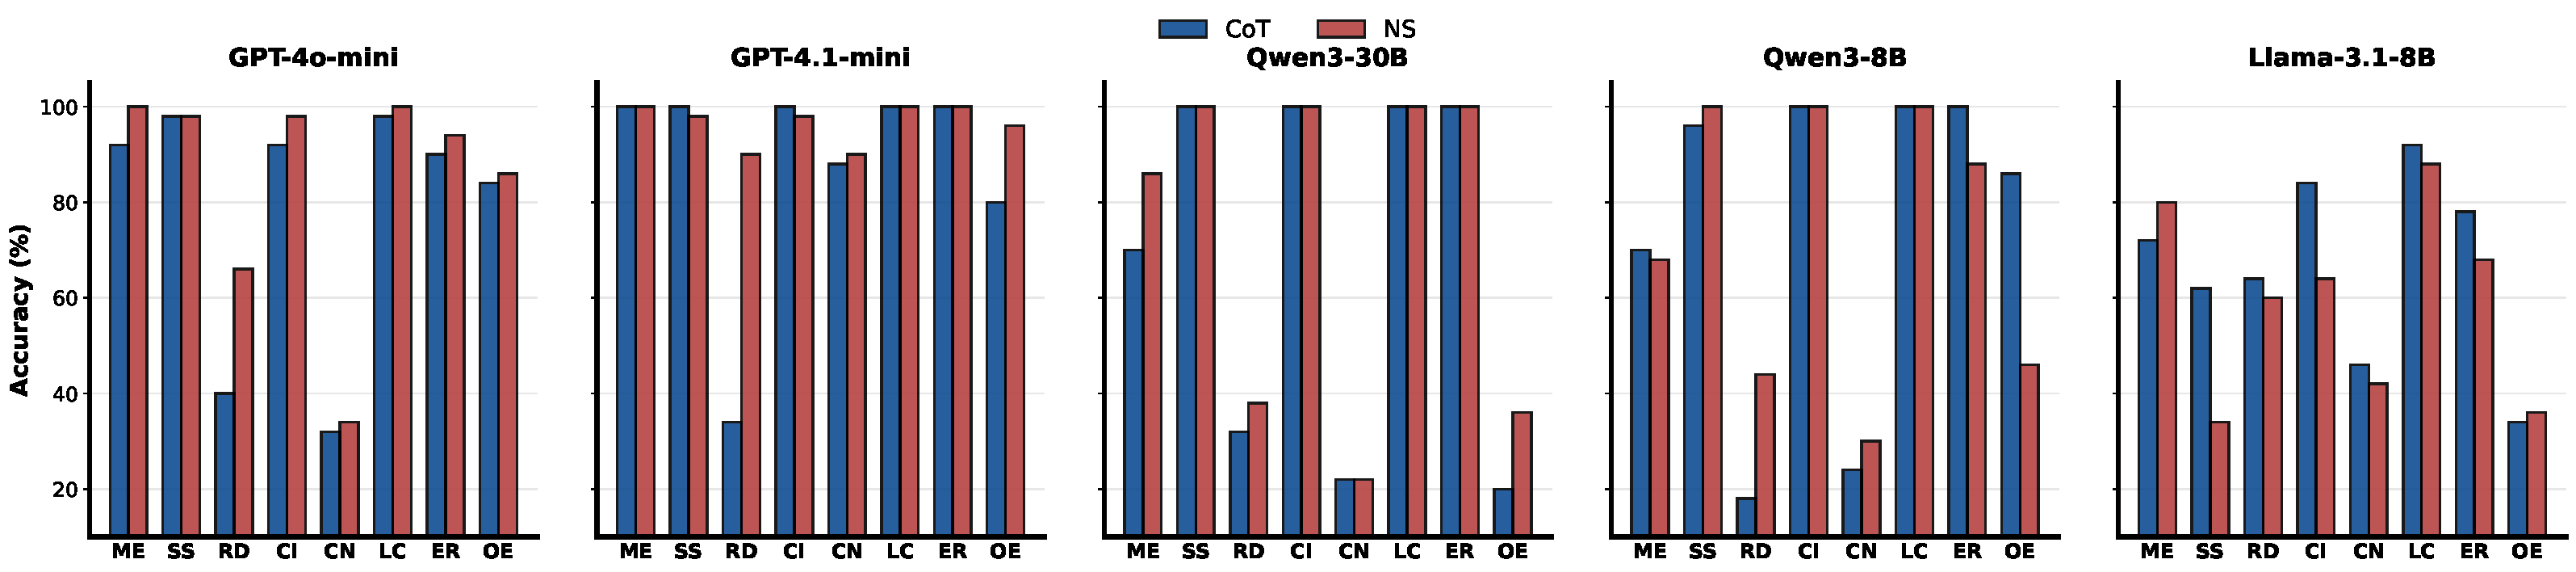
\includegraphics[width=\textwidth]{figures/fig_bar_d4.pdf}
    \caption{Per-category accuracy on strong-shortcut items at $d{=}4$. Blue = CoT, red = NS. Categories where NS exceeds CoT indicate effective shortcut activation; categories where NS falls below CoT indicate that estimation harms accuracy.}
    \label{fig:bar_d4}
\end{figure*}

The bar charts reveal qualitatively distinct profiles across models.
GPT-4o-mini and GPT-4.1-mini show NS improvements on most categories, with ME and LC reaching near-ceiling under NS.
Qwen3-30B and Qwen3-8B show NS benefits on ME and SS but drops on CN, LC, ER, and OE.
Llama-3.1-8B shows NS below CoT on most categories.

To account for differing CoT baselines across categories, Figure~\ref{fig:radar_norm} presents the normalized improvement $({\text{NS}} - {\text{CoT}}) / (1 - {\text{CoT}})$, measuring what fraction of the remaining accuracy gap NS captures.
GPT-4o-mini shows the broadest improvement profile, while Llama-3.1-8B is consistently negative.

\begin{figure}[t]
    \centering
    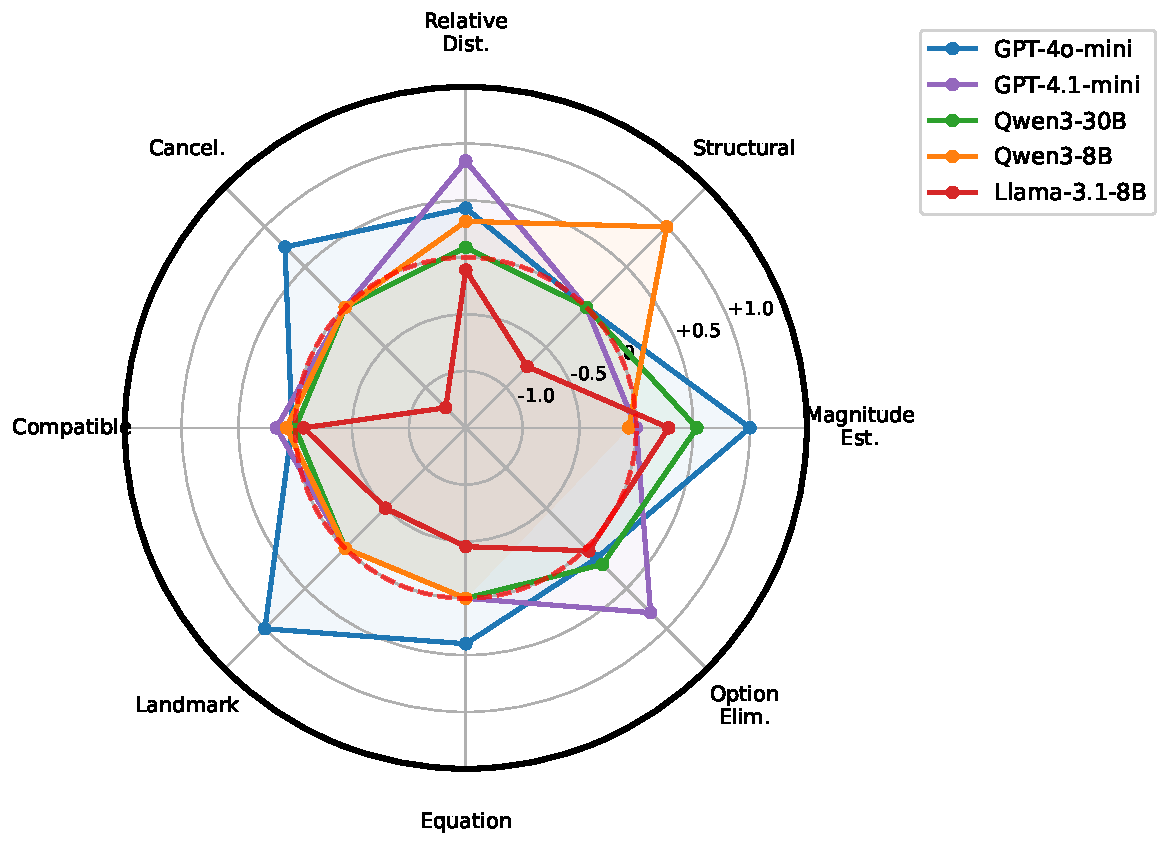
\includegraphics[width=0.7\textwidth]{figures/fig_radar_normalized_d4.pdf}
    \caption{Normalized NS improvement at $d{=}4$: $(\text{NS}-\text{CoT})/(1-\text{CoT})$. Values of $+1$ mean NS closes the entire remaining gap; $0$ means no change; negative means NS hurts. Red dashed line = zero.}
    \label{fig:radar_norm}
\end{figure}

These profiles suggest that number sense is not a single axis along which models can be ranked, but rather a multi-dimensional construct.
A model that excels at one shortcut type may perform at or below baseline on another.

\paragraph{Where NS hurts accuracy.}
NS reduces strong-item accuracy in several categories at $d{=}4$: option\_elimination ($-$44pp for Qwen3-8B), landmark\_comparison ($-$16pp), equation\_reasoning ($-$12pp), and magnitude\_estimation ($-$10pp).
These share a common trait: they require exact arithmetic or careful multi-step reasoning where estimation introduces fatal errors.
For equation reasoning, NS approximation compounds rounding errors (e.g., $3032+2697\approx5700$, but $5700-3391=2309$ instead of the exact 2338).
For option elimination with close distractors differing by 1--4 in the last digit, estimation cannot distinguish options.
By contrast, NS helps most on relative\_distance (+22pp for Qwen3-8B; +24pp for GPT-4o-mini), where CoT's extended reasoning introduces unnecessary computation.

Figures~\ref{fig:bar_d2}--\ref{fig:bar_d16} extend the per-category analysis to all digit scales, confirming that $d{=}4$ produces the most pronounced model-differentiated effects.

\begin{figure*}[t]
    \centering
    \begin{minipage}{0.49\textwidth}\centering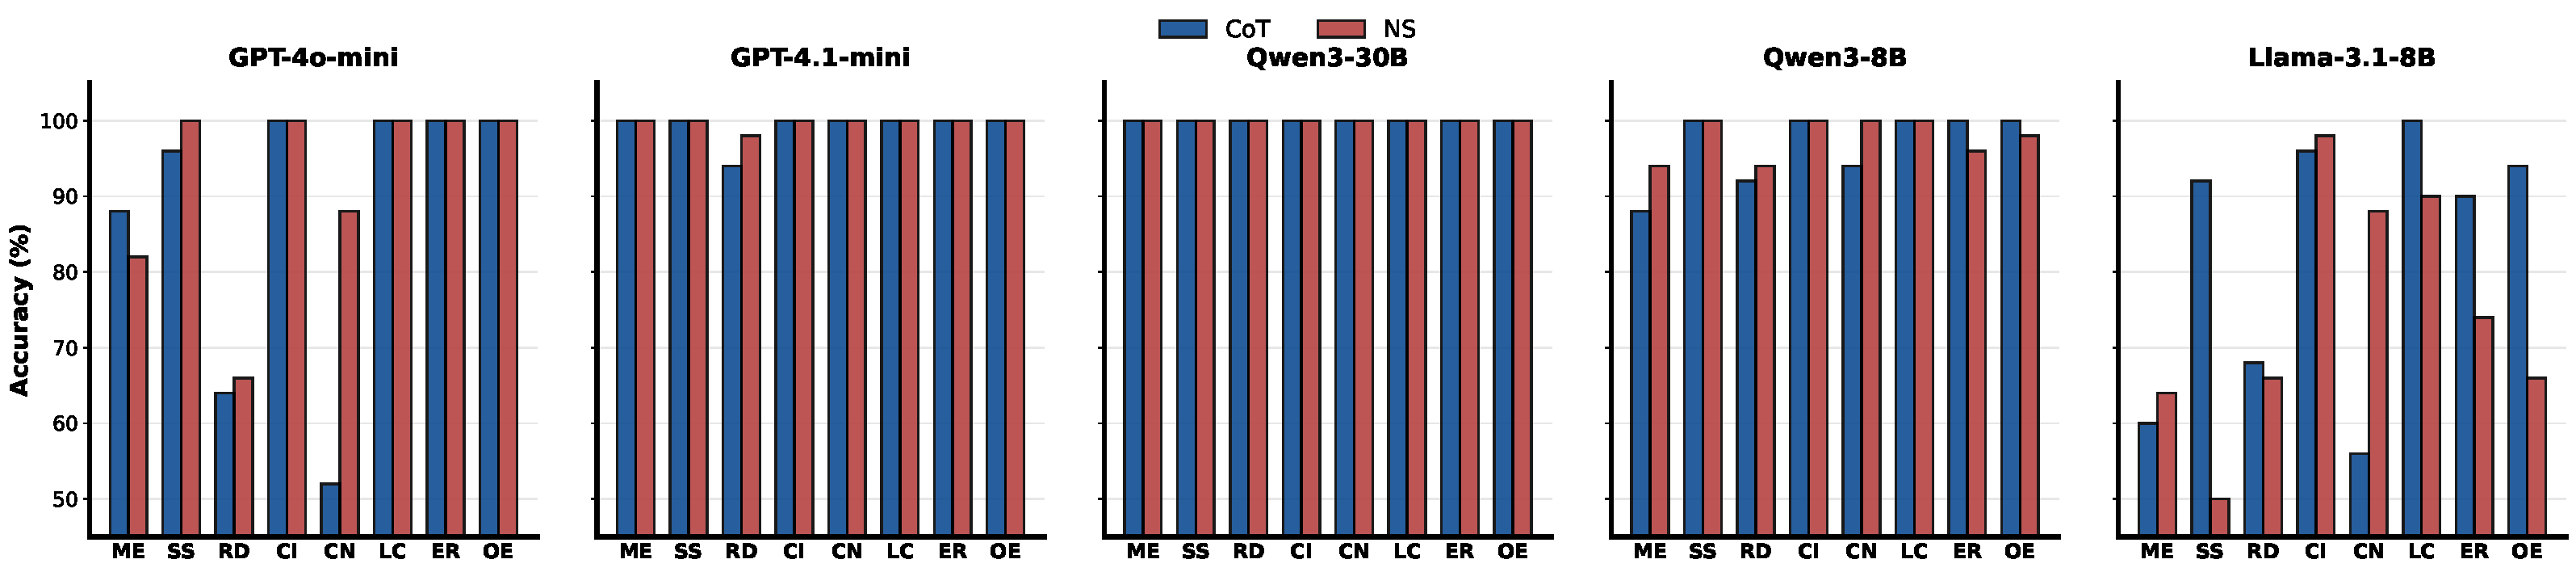
\includegraphics[width=\textwidth]{figures/fig_bar_d2.pdf}\caption{$d{=}2$}\label{fig:bar_d2}\end{minipage}
    \hfill
    \begin{minipage}{0.49\textwidth}\centering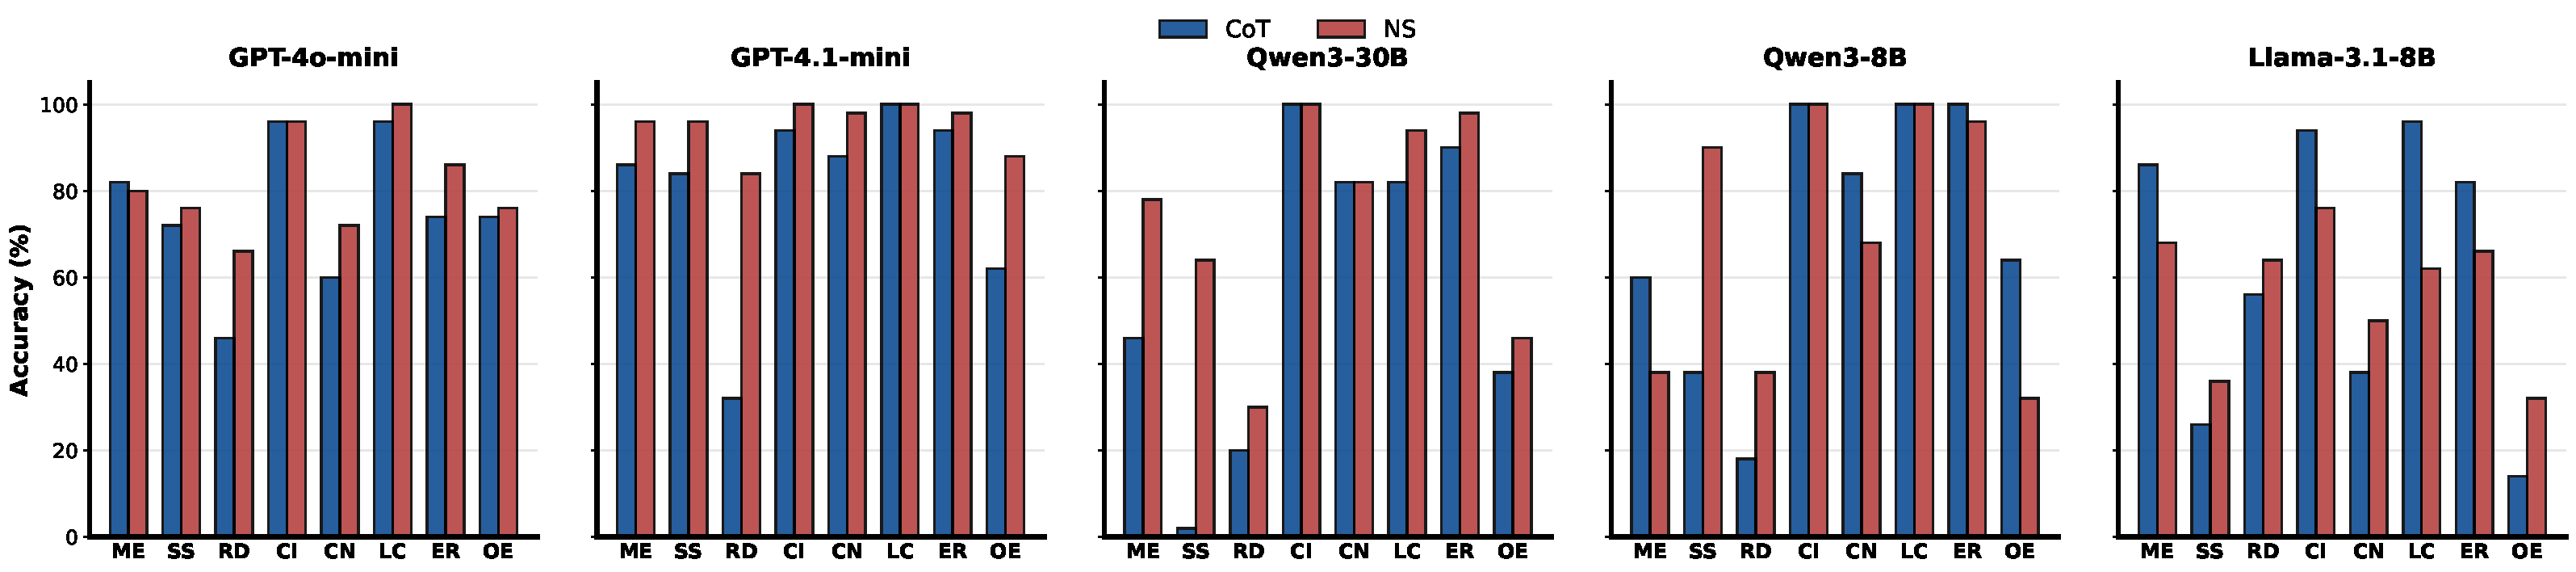
\includegraphics[width=\textwidth]{figures/fig_bar_d8.pdf}\caption{$d{=}8$}\label{fig:bar_d8}\end{minipage}
    \\[6pt]
    \begin{minipage}{0.49\textwidth}\centering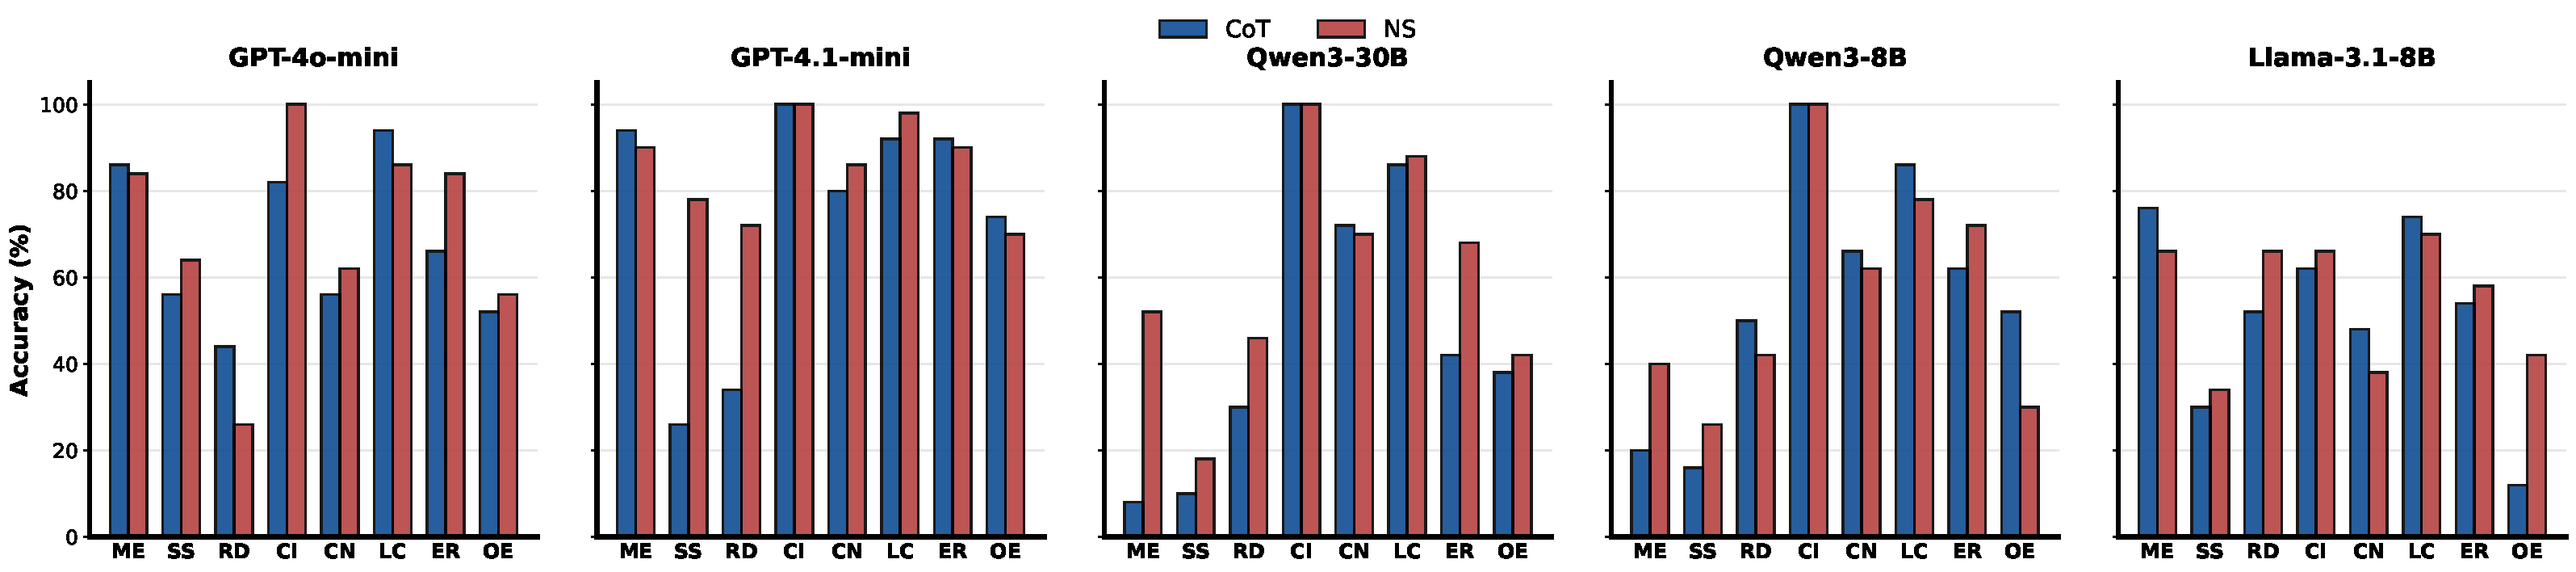
\includegraphics[width=\textwidth]{figures/fig_bar_d16.pdf}\caption{$d{=}16$}\label{fig:bar_d16}\end{minipage}
\end{figure*}

% ─────────────────────────────────────────────────────────────────────────────
\subsection{MATH-500 Number-Sense Analysis (Preliminary)}
\label{sec:math500}

As a preliminary test of whether number-sense prompting generalises beyond the controlled \textsc{SenseMath} items, we evaluate Qwen3-8B (base, no additional training) on MATH-500 \citep{hendrycks2021measuring}.

\paragraph{Annotation protocol.}
We partition MATH-500 into an \emph{NS-amenable} split and a \emph{computation-required} split using GPT-4.1-mini as a zero-shot classifier (temperature$\,{=}\,0$, $\texttt{max\_tokens}{=}10$).
Each problem is presented with the following prompt:
\begin{quote}
\small
\textit{You are classifying whether a math problem can benefit from Number Sense (NS) strategies (intuition, estimation, pattern recognition, magnitude reasoning, or structural shortcuts) or whether it fundamentally requires precise step-by-step algebraic/arithmetic computation. [\ldots] Reply with exactly one word: NS or COMP}
\end{quote}
This yields 171 NS-amenable problems (34.2\%) and 329 computation-required problems (65.8\%).
This classification task is structurally equivalent to our J1 judge task. The J1 accuracy across models (61--66\%) on the SenseMath dataset provides independent evidence that LLM-based classification of shortcut amenability is reliable.

\paragraph{Split results.}
On the NS-amenable split, Qwen3-8B under CoT achieves 84.8\% accuracy (avg.\ 262 tokens) versus NS at 83.0\% (avg.\ 235 tokens), a gap of only $\Delta = {-}1.8$pp with a 10.3\% token reduction.
On the computation-required split, CoT achieves 60.8\% (avg.\ 373 tokens) versus NS at 59.0\% (avg.\ 349 tokens), again $\Delta = {-}1.8$pp with a 6.4\% token reduction.

\paragraph{Key finding.}
Across both splits, the NS prompt causes minimal accuracy loss ($\leq 2$pp) on real MATH problems while consistently reducing token usage by 7--10\%.
This supports the practical viability of number-sense prompting as a drop-in efficiency improvement for math-capable models.

% ─────────────────────────────────────────────────────────────────────────────
\subsection{Strict Prompt Validation}
\label{sec:strict}

The Strict condition provides a negative control: by explicitly forbidding shortcuts, it should suppress shortcut-based reasoning and lower accuracy on strong-shortcut items.
We report Strict results for GPT-4o-mini only, because the open-weight models (Qwen, Llama) frequently truncate their Strict responses at the 512-token limit, rendering accuracy estimates unreliable.

\paragraph{GPT-4o-mini Strict results.}
At $d{=}4$, the gap between NS and Strict is substantial: NS achieves 84.5\% on strong items versus Strict's 90.5\%, but Strict control accuracy (87.2\%) far exceeds NS control accuracy (63.0\%).
Qualitative analysis of keyword frequencies in GPT-4o-mini outputs supports the interpretation: Strict responses contain shortcut-related keywords (e.g., ``approximately'', ``round'', ``cancel'') in only 11\% of responses, compared to 46\% under CoT and 87\% under NS.
This gradient, Strict $<$ CoT $<$ NS, is consistent with the view that CoT partially activates shortcuts (see \S\ref{sec:cot_strategy}), while NS maximally activates them and Strict effectively suppresses them.

\paragraph{Truncation caveat.}
For the three open-weight models, Strict prompting produces responses that exceed 512 tokens on 30--60\% of items (the instruction to show all arithmetic steps inflates response length).
Because truncated responses lack a \boxed{} answer and are scored as incorrect, accuracy under Strict is systematically deflated for these models.
We therefore treat Strict as a validation condition rather than a primary comparison, and restrict Strict-based analyses to GPT-4o-mini.

% ─────────────────────────────────────────────────────────────────────────────
\subsection{CoT Strategy Analysis}
\label{sec:cot_strategy}

An important nuance is that CoT does not uniformly produce pure computation.
Qualitative inspection of CoT responses reveals that models sometimes discover and apply shortcuts even without explicit prompting, particularly on strong-shortcut items with salient numerical structure.

For example, on a cancellation item ($3{,}456 + 7{,}891 - 7{,}889$), GPT-4o-mini's CoT response begins with standard addition but then states ``I notice $7{,}891 - 7{,}889 = 2$'' and immediately produces the correct answer.
Similarly, Qwen3-30B's CoT responses on structural-shortcut items frequently invoke the distributive law (``$99 \times 37 = (100-1) \times 37$'') without being prompted to look for such decompositions.

This spontaneous shortcut discovery under CoT has two implications.
First, it suggests that some degree of number-sense reasoning is embedded in these models' default behaviour and does not require explicit elicitation.
Second, and more importantly for interpreting our results, it means that the NS--CoT comparison is \emph{conservative}: the NS condition activates shortcuts that CoT does not, but CoT already activates some shortcuts on its own.
The NS--Strict comparison, where Strict suppresses even spontaneous shortcuts, produces a wider gap.

This conservatism strengthens the interpretation: even against a partially shortcut-aware CoT baseline, the NS prompt produces a measurable additional asymmetric effect on shortcut-amenable items.

\paragraph{Strategy-use quantification.}
To move beyond accuracy and directly measure strategy choice, we use GPT-4.1-mini as a judge to classify every model response as SHORTCUT or COMPUTATION across all five models and all digit scales.
The NS\% rows in Table~\ref{tab:main_results} report the results.
Under CoT, shortcut rates are low (20--39\% at $d{=}4$) with a consistent strong$>$control gap for Qwen3-30B and Qwen3-8B, confirming that shortcut-amenable items spontaneously elicit more shortcut reasoning.
NS prompting dramatically increases shortcut use to 68--86\% across all models, scales, and variants.
Crucially, the NS shortcut rate is similar on strong and control items (e.g., Qwen3-8B at $d{=}4$: 86\% strong, 88\% control).
This reveals the mechanism behind the accuracy asymmetry: NS induces shortcut strategies uniformly, but these strategies succeed on strong items (where valid shortcuts exist) and fail on control items (where no shortcut applies).

% ─────────────────────────────────────────────────────────────────────────────
\subsection{Judge and Generate Tasks}
\label{sec:judge_generate}

We evaluate declarative shortcut knowledge through Judge tasks and constructive shortcut ability through Generate tasks.

\paragraph{J1: Shortcut appropriateness.}
Models are asked whether a number-sense shortcut would be effective for a given problem (YES/NO), evaluated on 251 items after filtering.
GPT-4o-mini achieves the highest J1 accuracy (66.3\%), with perfect recognition of shortcut-amenable items (100\% on strong) but complete failure to reject non-shortcut items (0\% on control). It says YES to every item.
GPT-4.1-mini scores 65.3\% overall with a more balanced profile (89.1\% strong, 15.8\% control), suggesting better calibration at the cost of lower shortcut recognition.
Qwen3-8B follows at 65.0\% (97.8\% strong, 0\% control), exhibiting the same extreme YES bias as GPT-4o-mini.
Qwen3-30B scores 64.0\% (96.7\% strong, 4.0\% control), also strongly biased toward YES.
Llama-3.1-8B scores 61.3\% (82.6\% strong, 20.8\% control), showing a relatively more balanced profile among the tested models.
The near-zero control accuracy for most models reflects over-rationalization: given any problem, the model can construct a plausible shortcut strategy, making it unable to reject control items.

\paragraph{J2: Strategy identification.}
Given a problem and its solution, models classify whether the solution used a shortcut or computation strategy (SHORTCUT/COMPUTATION).
The J2 dataset comprises 80 verified items: 54 SHORTCUT cases drawn from NS responses on strong-shortcut items, and 26 COMPUTATION cases drawn from CoT responses on control items; all labels were confirmed by manual audit.
GPT-4.1-mini achieves the highest J2 accuracy (91.2\%), with balanced performance on both SHORTCUT (90.7\%) and COMPUTATION (92.3\%) identification.
GPT-4o-mini correctly identifies shortcuts in 94.0\% of cases but misclassifies computation as shortcut in 42\% of cases, suggesting a liberal bias toward labelling solutions as shortcut-based.

\paragraph{G2: Problem generation.}
Models generate novel shortcut/control problem pairs from a category description and one example, verified by 6 deterministic code checks.
Qwen3-30B leads at 25\% pass rate, followed by Qwen3-8B (20\%), GPT-4.1-mini (18\%), GPT-4o-mini (9\%), and Llama-3.1-8B (2\%). All models are evaluated on 96 prompts (8 categories $\times$ 12).
The primary bottleneck is constructing expressions where a valid shortcut exists: the shortcut-existence check fails on 51\% of generated items across all models.
A common failure mode is generating numerically plausible strong items where the intended structure (e.g., operand near a power of 10) is too weak to qualify as a genuine shortcut.

Table~\ref{tab:judge} and Table~\ref{tab:generate} present the full results.

\begin{table}[t]
\centering
\small
\caption{Judge task results. J1: shortcut appropriateness (251 items). J2: strategy identification (80 items). \textcolor{green!60!black}{Green}/\textcolor{red!70!black}{red} = gap from ideal (100\% for strong, 100\% for control).}
\label{tab:judge}
\begin{tabular}{llrrr}
\toprule
Task & Model & Overall (\%) & Strong (\%) & Control (\%) \\
\midrule
J1 & GPT-4o-mini  & 66 & 100 & 0 \textcolor{red!70!black}{\scriptsize $-$100} \\
   & GPT-4.1-mini & 65 & 89 \textcolor{red!70!black}{\scriptsize $-$11} & 16 \textcolor{red!70!black}{\scriptsize $-$84} \\
   & Qwen3-8B     & 65 & 98 \textcolor{red!70!black}{\scriptsize $-$2} & 0 \textcolor{red!70!black}{\scriptsize $-$100} \\
   & Qwen3-30B    & 64 & 97 \textcolor{red!70!black}{\scriptsize $-$3} & 4 \textcolor{red!70!black}{\scriptsize $-$96} \\
   & Llama-3.1-8B & 61 & 83 \textcolor{red!70!black}{\scriptsize $-$17} & 21 \textcolor{red!70!black}{\scriptsize $-$79} \\
\midrule
 & & Overall (\%) & SHORTCUT (\%) & COMP (\%) \\
\midrule
J2 & GPT-4.1-mini & 91 & 91 & 92 \\
   & GPT-4o-mini  & 70 \textcolor{red!70!black}{\scriptsize $-$21} & 94 \textcolor{green!60!black}{\scriptsize +3} & 58 \textcolor{red!70!black}{\scriptsize $-$34} \\
\bottomrule
\end{tabular}
\end{table}

\begin{table}[t]
\centering
\small
\caption{G2 problem generation: per-check pass rates (\%) and 6/6 pass. All models evaluated on 96 prompts (8 categories $\times$ 12). \textcolor{green!60!black}{Green}/\textcolor{red!70!black}{red} = delta from top model per column.}
\label{tab:generate}
\setlength{\tabcolsep}{3pt}
\begin{tabular}{l r rrrrrr r}
\toprule
Model & Fmt & S.Ans & C.Ans & SC.Ex & C.Blk & Fam & Nov & Pass \\
\midrule
Qwen3-30B    & 96 & 65 & 73 & 66 & 87 & 76 & 96 & 23/96 \\
Qwen3-8B     & 100 & 69 \textcolor{green!60!black}{\scriptsize+4} & 64 \textcolor{red!70!black}{\scriptsize$-$9} & 55 \textcolor{red!70!black}{\scriptsize$-$11} & 83 \textcolor{red!70!black}{\scriptsize$-$4} & 71 \textcolor{red!70!black}{\scriptsize$-$5} & 99 \textcolor{green!60!black}{\scriptsize+3} & 19/96 \\
GPT-4.1-mini & 100 & 70 \textcolor{green!60!black}{\scriptsize+5} & 79 \textcolor{green!60!black}{\scriptsize+6} & 67 \textcolor{green!60!black}{\scriptsize+1} & 80 \textcolor{red!70!black}{\scriptsize$-$7} & 75 \textcolor{red!70!black}{\scriptsize$-$1} & 94 \textcolor{red!70!black}{\scriptsize$-$2} & 17/96 \\
GPT-4o-mini  & 100 & 58 \textcolor{red!70!black}{\scriptsize$-$7} & 48 \textcolor{red!70!black}{\scriptsize$-$25} & 46 \textcolor{red!70!black}{\scriptsize$-$20} & 82 \textcolor{red!70!black}{\scriptsize$-$5} & 73 \textcolor{red!70!black}{\scriptsize$-$3} & 88 \textcolor{red!70!black}{\scriptsize$-$8} & 9/96 \\
Llama-3.1-8B & 100 & 51 \textcolor{red!70!black}{\scriptsize$-$14} & 46 \textcolor{red!70!black}{\scriptsize$-$27} & 38 \textcolor{red!70!black}{\scriptsize$-$28} & 83 \textcolor{red!70!black}{\scriptsize$-$4} & 52 \textcolor{red!70!black}{\scriptsize$-$24} & 90 \textcolor{red!70!black}{\scriptsize$-$6} & 2/96 \\
\bottomrule
\end{tabular}
\end{table}


\begin{figure}[t]
\centering
\small
\fbox{\parbox{0.93\columnwidth}{%
\textbf{G2 Pass} (Qwen3-30B, magnitude\_estimation).\\
Strong: $10{,}200 \times 9{,}800 = 99{,}960{,}000$ \checkmark\quad
Control: $4{,}321 \times 5{,}678 = 24{,}537{,}538$ \checkmark\\
Both operands near $10^4$ in strong $\Rightarrow$ shortcut exists; control operands far from round numbers $\Rightarrow$ shortcut blocked. All 6 checks pass.\\[6pt]
%
\textbf{G2 Fail} (Qwen3-30B, magnitude\_estimation).\\
Strong: $10{,}200 \times 9{,}850$; model claims $= 100{,}000{,}000$, actual $= 100{,}470{,}000$ \ding{55}\\
The model rounded too aggressively ($10{,}200 \approx 10{,}000$, $9{,}850 \approx 10{,}000$) and reported the estimate as the exact answer. The shortcut-existence check passes, but the answer-correctness check fails.
}}
\caption{G2 generation examples. Pass: model produces a valid shortcut/control pair. Fail: model confuses its own shortcut estimate with the exact answer.}
\label{fig:g2_case}
\end{figure}

% ─────────────────────────────────────────────────────────────────────────────
\subsection{Post-Training (Preliminary): Can Number Sense Be Trained?}
\label{sec:training}

The prompting experiments establish that number-sense shortcuts can be elicited at inference time.
A natural follow-up asks whether targeted \emph{training} can internalize number-sense reasoning more durably.
We present a proof-of-concept study using Qwen3-8B fine-tuned with Direct Preference Optimization (DPO) on 500 MATH problems, pairing NS-style shortcut solutions (generated by GPT-5.1) as preferred responses against verbose CoT solutions as rejected responses.
Training uses LoRA (rank 8, all linear layers) with LLaMA-Factory; full hyperparameters appear in the supplementary material.

\paragraph{Combined-DPO results.}
After training, Qwen3-8B achieves 68.0\% accuracy under NS prompting on a held-out 200-problem MATH evaluation set, an improvement of ${+}3.0$pp over the base model (65.0\%).
Average token usage increases modestly to 375 tokens from 340 in the base model, reflecting slightly longer shortcut explanations in the fine-tuned outputs.

\paragraph{Out-of-distribution (OOD) generalization.}
To verify that training on number-sense examples does not harm general capabilities, we evaluate the fine-tuned model on 7 standard benchmarks.
All results fall within $\pm 4$pp of the base model: BBH 73.8\%$\to$69.8\%, ARC 87.0\%$\to$87.0\%, and similar small changes across the remaining five benchmarks.
Table~\ref{tab:ood} presents the full OOD comparison.

\begin{table}[t]
\centering
\caption{Out-of-distribution benchmark results after 500-example training. Most variants fall within $\pm$4pp of base, confirming no catastrophic forgetting.}
\label{tab:ood}
\small
\setlength{\tabcolsep}{3.5pt}
\begin{tabular}{ll ccccccc}
\toprule
Model & Variant & BBH & ARC & GPQA & MMLU-P & MedQA & LogiQA & CSQA \\
\midrule
Qwen3-8B & Base         & 73.8 & 87.0 & 34.6 & 31.8 & 61.4 & 50.5 & 80.8 \\
         & NS-DPO       & 73.8 & 87.0 & 31.2 & 31.4 & 59.4 & 46.9 & 80.8 \\
         & Baseline-DPO & 73.6 & 86.6 & 34.6 & 31.8 & 59.0 & 47.9 & 80.7 \\
         & NS-SFT       & 73.6 & 86.6 & 33.7 & 32.6 & 60.4 & 48.4 & 80.7 \\
         & CoT-SFT      & 73.4 & 86.3 & 32.8 & 30.6 & 60.6 & 48.7 & 80.9 \\
         & Comb-SFT     & --- & --- & --- & --- & --- & --- & --- \\
         & Comb-DPO     & 69.8 & 87.0 & 35.0 & 28.4 & 62.2 & 51.0 & 80.0 \\
\midrule
Llama-3-8B & Base       & 50.2 & 80.3 & 29.2 & 19.2 & 60.6 & 41.6 & 75.4 \\
           & NS-DPO     & 49.8 & 80.6 & 28.6 & 19.4 & 59.6 & 42.4 & 75.7 \\
           & Baseline-DPO & 50.2 & 80.3 & 28.8 & 18.4 & 60.2 & 42.1 & 75.7 \\
           & NS-SFT     & 50.6 & 80.3 & 28.8 & 18.8 & 60.4 & 42.4 & 75.8 \\
           & CoT-SFT    & 50.4 & 80.3 & 29.9 & 19.0 & 60.4 & 41.8 & 75.9 \\
           & Comb-SFT   & 54.4 & 82.6 & 27.9 & 17.4 & 59.4 & 40.9 & 74.6 \\
           & Comb-DPO   & 54.4 & 82.3 & 29.2 & 18.0 & 59.6 & 41.0 & 74.5 \\
\bottomrule
\end{tabular}
\end{table}


\begin{table}[t]
\centering
\caption{In-domain results on the 200-problem eval set (500-example training). NS Rate = fraction of responses using number-sense strategy; Avg Tok = average response tokens. Best accuracy per model per prompt condition is \textbf{bold}.}
\label{tab:training}
\small
\begin{tabular}{ll l ccc}
\toprule
Model & Variant & Prompt & NS Rate & Accuracy & Avg Tok \\
\midrule
Qwen3-8B   & Base          & CoT & 10.0\% & 64.5\%          & 376 \\
(nothink)  & Base          & NC  & 36.5\% & 65.0\%          & 340 \\
           & NS-DPO        & CoT & 11.5\% & \textbf{67.0\%} & 372 \\
           & NS-DPO        & NC  & 33.5\% & 64.0\%          & 350 \\
           & Baseline-DPO  & CoT &  8.5\% & 66.0\%          & 374 \\
           & Baseline-DPO  & NC  & 34.5\% & 60.0\%          & 350 \\
           & NS-SFT        & CoT & 11.5\% & 66.0\%          & 369 \\
           & NS-SFT        & NC  & 32.5\% & 64.0\%          & 348 \\
           & CoT-SFT       & CoT & 11.5\% & 64.0\%          & 373 \\
           & CoT-SFT       & NC  & 34.5\% & 63.0\%          & 351 \\
           & Combined-SFT  & CoT & 11.5\% & 63.0\%          & 392 \\
           & Combined-SFT  & NC  & 22.0\% & 65.5\%          & 372 \\
           & Combined-DPO  & CoT & 11.0\% & 62.5\%          & 395 \\
           & Combined-DPO  & NC  & 23.5\% & \textbf{68.0\%} & 375 \\
\midrule
Llama-3-8B & Base          & CoT &  5.5\% & 21.5\%          & 363 \\
           & Base          & NC  & 44.5\% & 15.5\%          & 269 \\
           & NS-DPO        & CoT &  3.5\% & 22.5\%          & --- \\
           & NS-DPO        & NC  & 48.0\% & 17.0\%          & --- \\
           & Baseline-DPO  & CoT &  4.5\% & 18.5\%          & --- \\
           & Baseline-DPO  & NC  & 51.0\% & 17.0\%          & --- \\
           & NS-SFT        & CoT &  3.5\% & 24.0\%          & 398 \\
           & NS-SFT        & NC  & 57.5\% & 16.0\%          & 285 \\
           & CoT-SFT       & CoT &  3.0\% & 25.0\%          & 379 \\
           & CoT-SFT       & NC  & 59.0\% & 19.0\%          & 292 \\
           & Combined-SFT  & CoT &  4.0\% & \textbf{37.5\%} & 321 \\
           & Combined-SFT  & NC  & 16.0\% & 31.5\%          & 286 \\
           & Combined-DPO  & CoT &  4.5\% & 36.5\%          & 325 \\
           & Combined-DPO  & NC  & 12.0\% & 30.0\%          & 288 \\
\bottomrule
\end{tabular}
\end{table}


\paragraph{Conclusion.}
Small-scale DPO training (500 examples) on number-sense-preferred solutions improves shortcut exploitation by up to 3pp without degrading generalization across seven diverse OOD benchmarks (Table~\ref{tab:ood}).
This demonstrates that number sense is a trainable capability, and that the prompt-level effects observed in the main experiments can be amplified through targeted post-training.
